\begin{figure}[!htbp]\centering
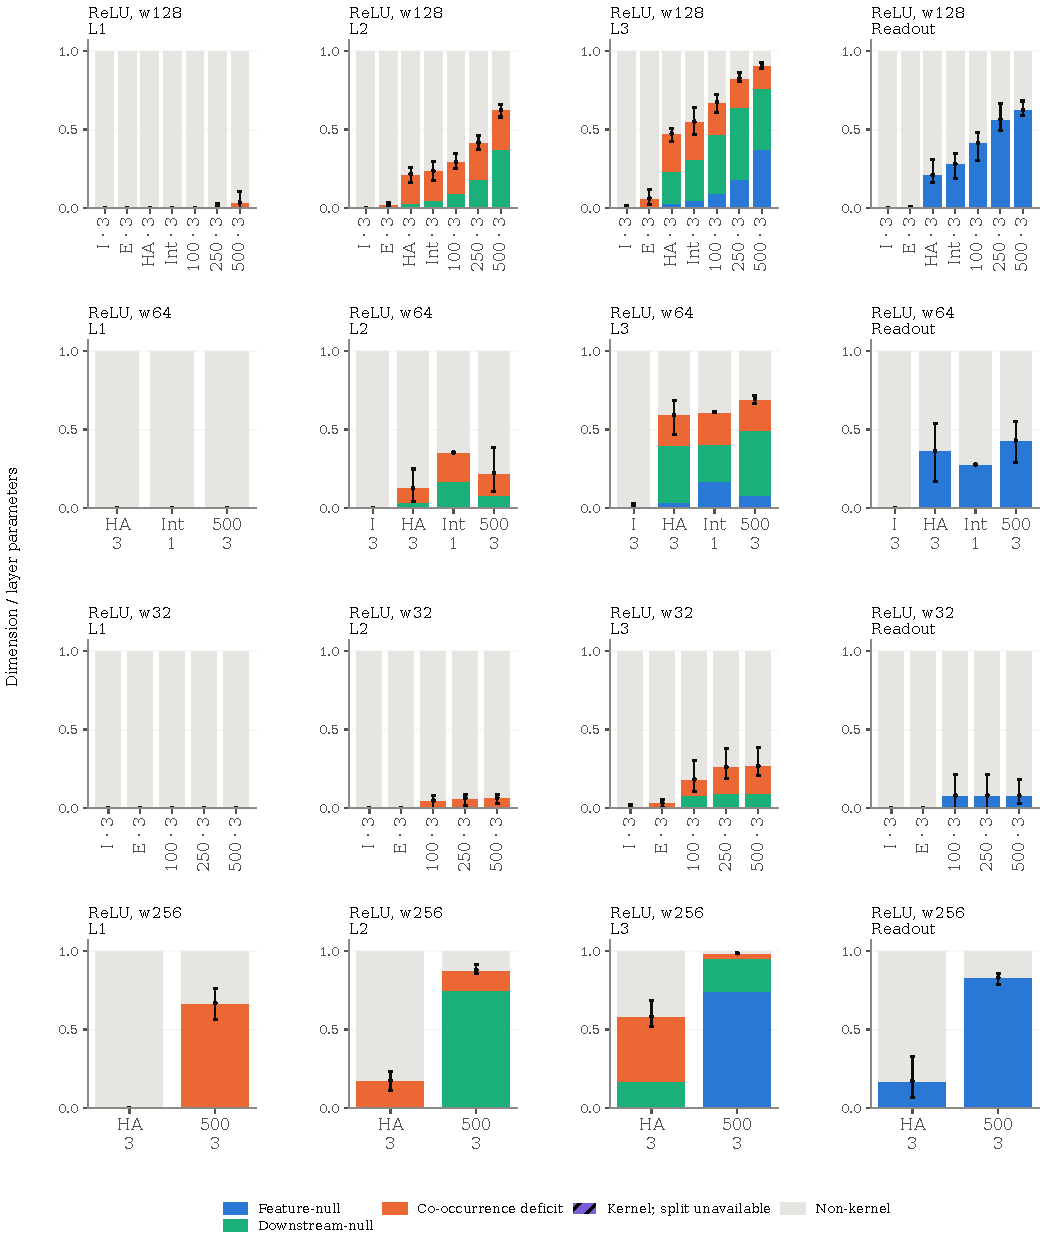
\includegraphics[width=6.272in]{compact_atomic_00.pdf}
\caption{Atomic decomposition across the indicated models and layers. Models use MNIST unless labeled SVHN; w and d denote width and hidden depth. Panels show a layer across stages, or all editable layers at the stated endpoint. Heights are fractions of layer parameters; bars average seeds and whiskers span their kernel fractions. Seed counts follow each stage label, on a second line or after a dot. I, E, HA, Int and Val denote initialization, early fitting, high accuracy, interpolation and validation selection; numbers denote fixed epochs. Stages are grouped by milestone and then fixed epoch. For reduced-data models, $n$ is the retraining or analysis-set size as titled. Hatched kernels have no measured component split. Counts use the $10^{-9}$ rank rule; GELU late-stage counts and layers without a spectral gap remain threshold-dependent.}\label{fig:c-atomic-0}
\end{figure}
\begin{figure}[!htbp]\centering
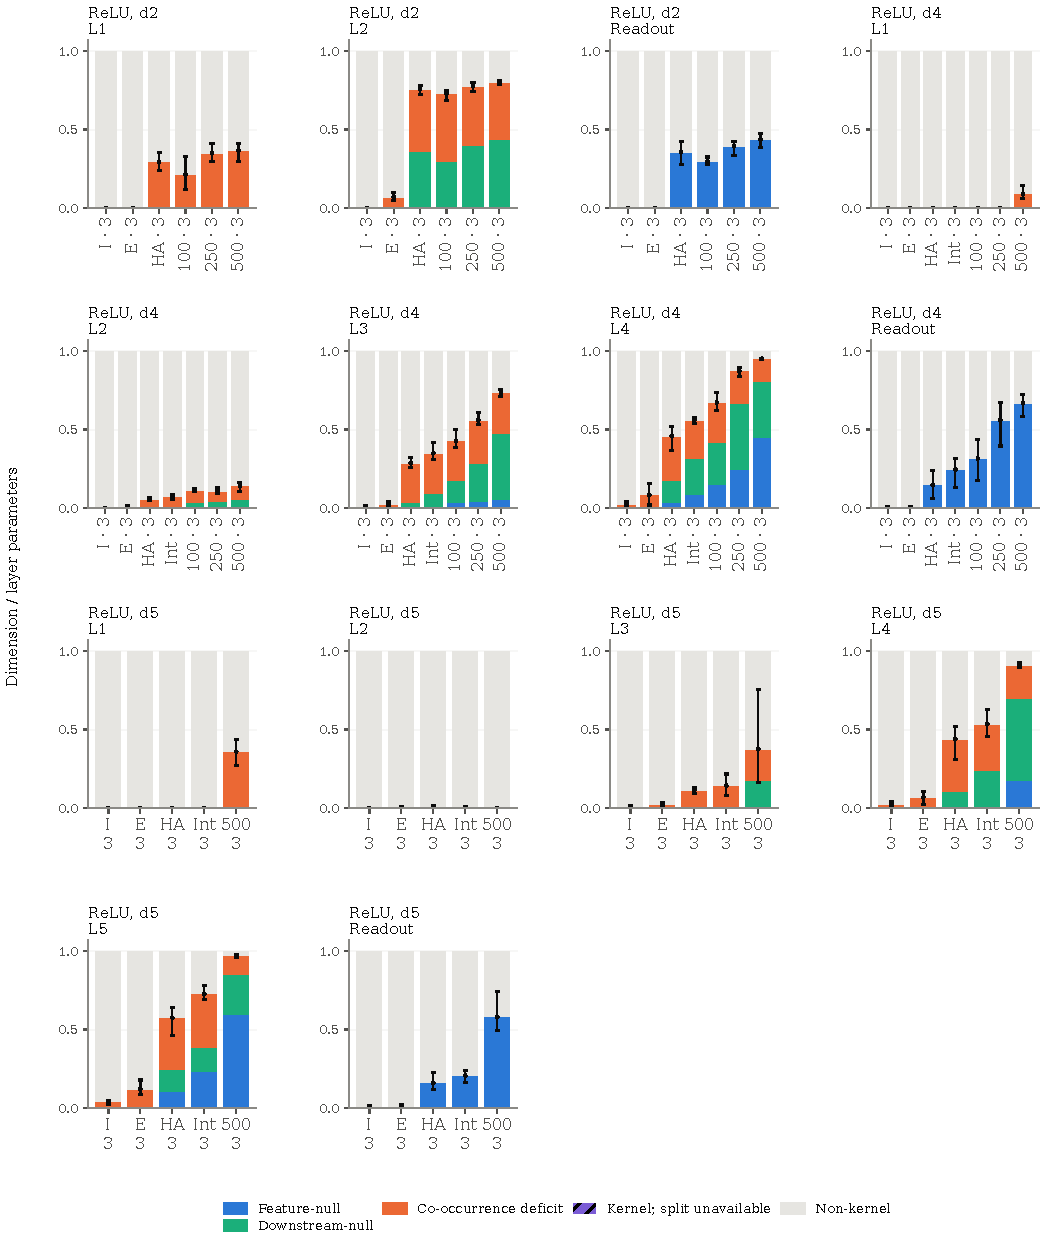
\includegraphics[width=6.272in]{compact_atomic_01.pdf}
\caption{Atomic decomposition across the indicated models and layers. Models use MNIST unless labeled SVHN; w and d denote width and hidden depth. Panels show a layer across stages, or all editable layers at the stated endpoint. Heights are fractions of layer parameters; bars average seeds and whiskers span their kernel fractions. Seed counts follow each stage label, on a second line or after a dot. I, E, HA, Int and Val denote initialization, early fitting, high accuracy, interpolation and validation selection; numbers denote fixed epochs. Stages are grouped by milestone and then fixed epoch. For reduced-data models, $n$ is the retraining or analysis-set size as titled. Hatched kernels have no measured component split. Counts use the $10^{-9}$ rank rule; GELU late-stage counts and layers without a spectral gap remain threshold-dependent.}\label{fig:c-atomic-1}
\end{figure}
\begin{figure}[!htbp]\centering
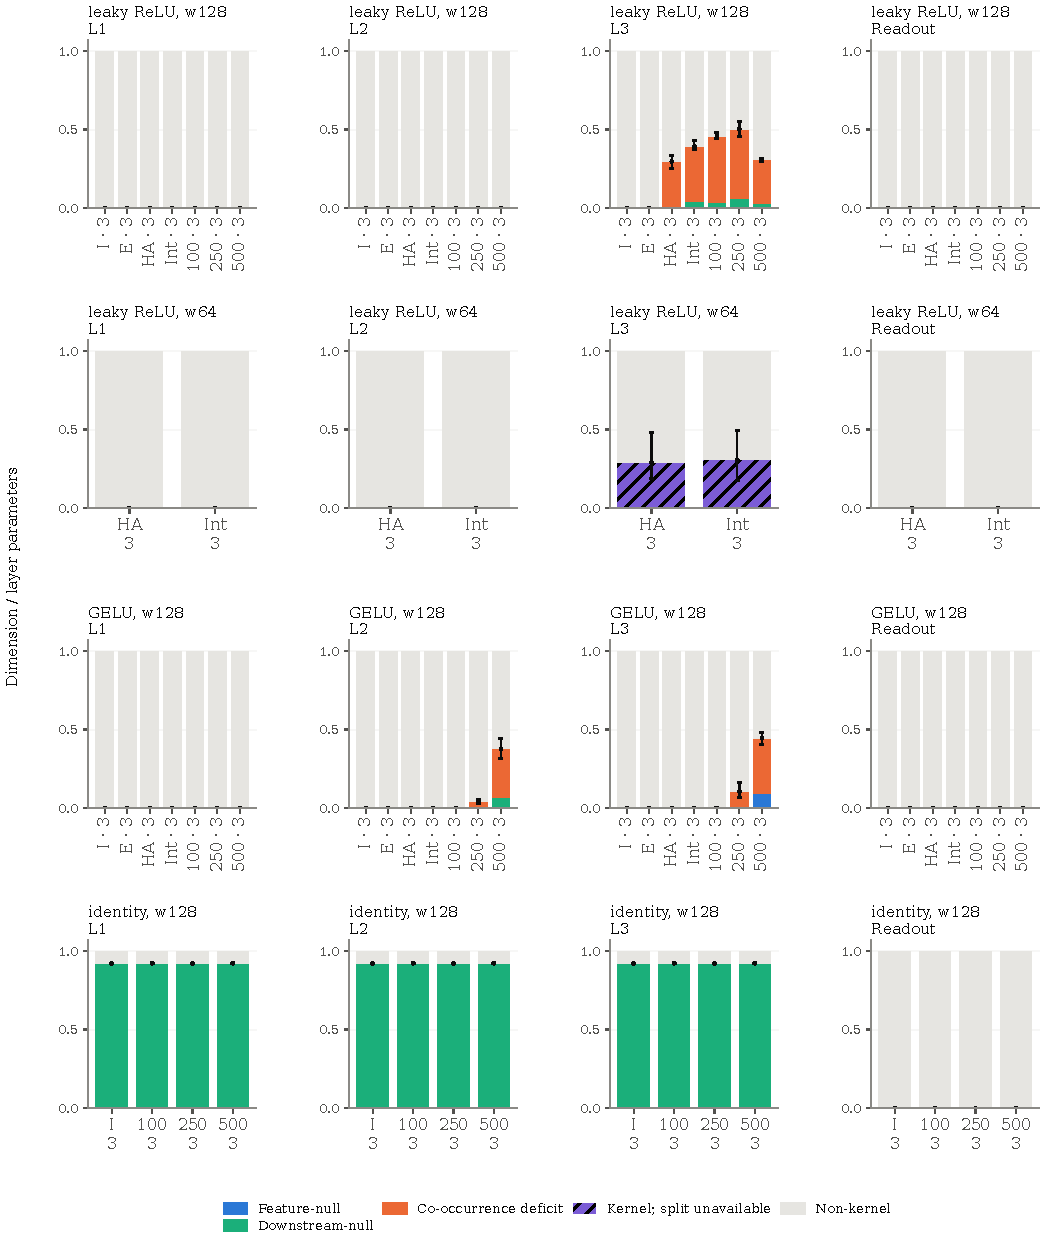
\includegraphics[width=6.272in]{compact_atomic_02.pdf}
\caption{Atomic decomposition across the indicated models and layers. Models use MNIST unless labeled SVHN; w and d denote width and hidden depth. Panels show a layer across stages, or all editable layers at the stated endpoint. Heights are fractions of layer parameters; bars average seeds and whiskers span their kernel fractions. Seed counts follow each stage label, on a second line or after a dot. I, E, HA, Int and Val denote initialization, early fitting, high accuracy, interpolation and validation selection; numbers denote fixed epochs. Stages are grouped by milestone and then fixed epoch. For reduced-data models, $n$ is the retraining or analysis-set size as titled. Hatched kernels have no measured component split. Counts use the $10^{-9}$ rank rule; GELU late-stage counts and layers without a spectral gap remain threshold-dependent.}\label{fig:c-atomic-2}
\end{figure}
\begin{figure}[!htbp]\centering
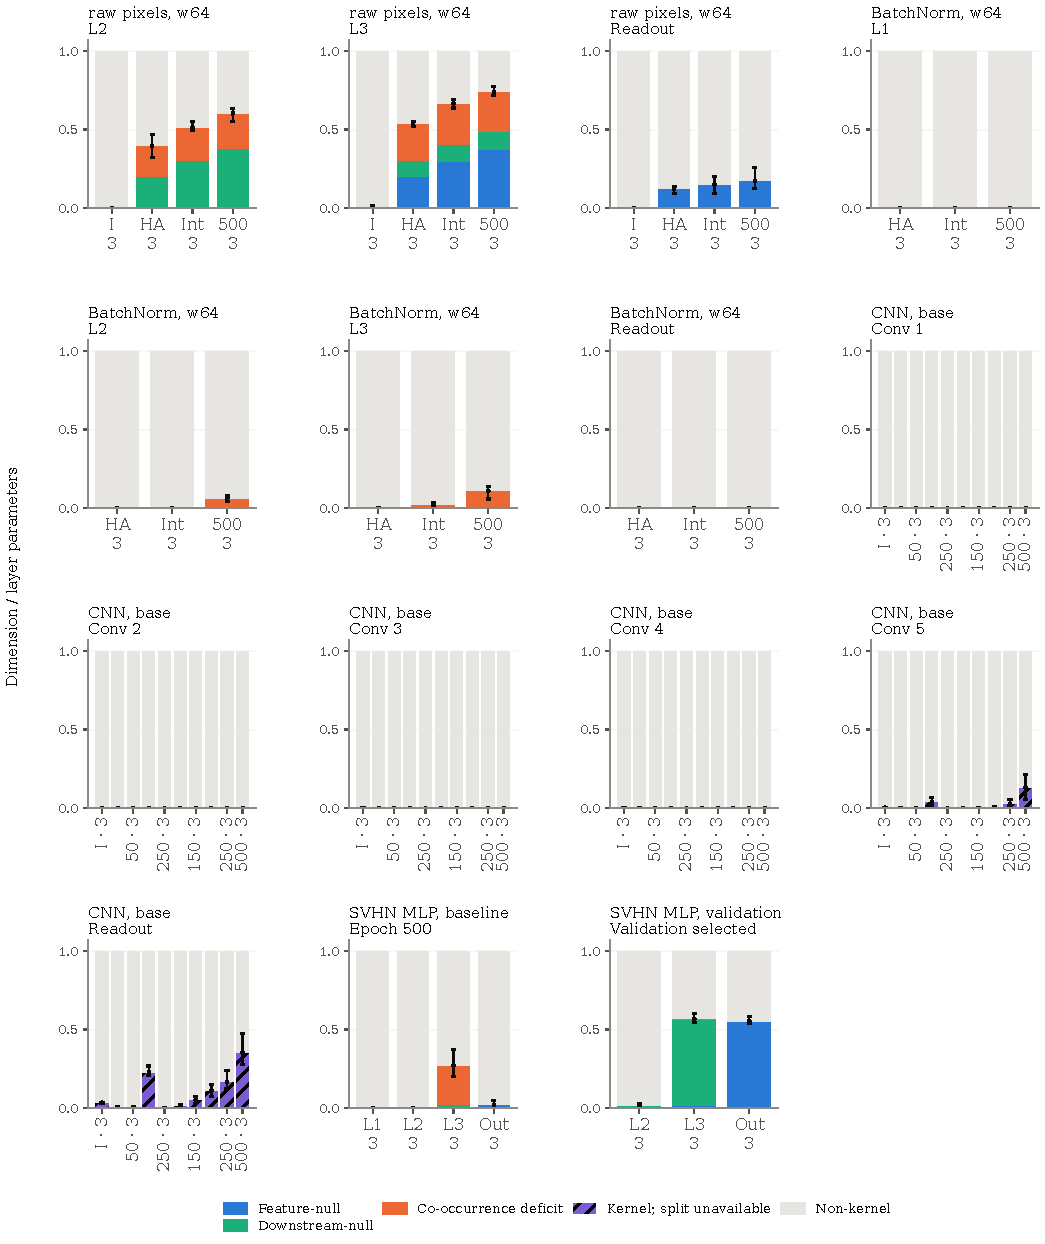
\includegraphics[width=6.272in]{compact_atomic_03.pdf}
\caption{Atomic decomposition across the indicated models and layers. Models use MNIST unless labeled SVHN; w and d denote width and hidden depth. Panels show a layer across stages, or all editable layers at the stated endpoint. Heights are fractions of layer parameters; bars average seeds and whiskers span their kernel fractions. Seed counts follow each stage label, on a second line or after a dot. I, E, HA, Int and Val denote initialization, early fitting, high accuracy, interpolation and validation selection; numbers denote fixed epochs. Stages are grouped by milestone and then fixed epoch. For reduced-data models, $n$ is the retraining or analysis-set size as titled. Hatched kernels have no measured component split. Counts use the $10^{-9}$ rank rule; GELU late-stage counts and layers without a spectral gap remain threshold-dependent.}\label{fig:c-atomic-3}
\end{figure}
\FloatBarrier
